% =============================================================================
% DOCUMENT CLASS , ENCODING , TITLE -------------------------------------- {{{

\documentclass[a4paper,twocolumn,10pt]{article}
\setlength{\columnsep}{20pt}
%\setlength{\columnseprule}{1pt}
\usepackage[utf8]{inputenc}
\usepackage[english]{babel}

\title{This is title for this document}
\author{John Doestar}
\date{\today}

% }}}
% FONTS ------------------------------------------------------------------ {{{

\usepackage{courier}     % courier font
%\usepackage{fontawesome} % font awesome glyphs
\usepackage{setspace}    % inter line spacing
\singlespacing           % set spacing to single spaced

% \onehalfspacing
% \doublespacing
% \setstretch{1.1}


% }}}
% PAGE FORMAT ------------------------------------------------------------ {{{

\usepackage[document]{ragged2e} % Text alignment package
\usepackage{enumitem}           %
\usepackage{geometry}           %
\geometry{
	a4paper,
	total = {170mm,257mm},
	top=20mm,
	left=20mm,
	right=20mm,
	bottom=20mm
}


\usepackage[switch]{lineno} % switch allows line numbers on alternating sides
%\usepackage[switch,displaymath,mathlines]{lineno}
%\modulolinenumbers[5]
\linenumberfont{\normalfont\large\sffamily}
\renewcommand{\thelinenumber}{\color{gray}\arabic{linenumber}}

\setlength\linenumbersep{0.5cm}


% }}}
% TEXT FORMAT ------------------------------------------------------------ {{{

\usepackage[activate={true,nocompatibility},
final,
tracking=true,
kerning=true,
spacing=true,
factor=1100,
stretch=10,
shrink=10]{microtype}
% prevents a certiain amount of overfull hbox badness
% helps with other margin stuff

\usepackage{verbatim}
\makeatletter
\newcommand{\verbatimfont}[1]{\def\verbatim@font{#1}}%
\makeatother%\verbatimfont{courier}

\usepackage{type1cm}  % Allows font resizing
\usepackage{lettrine} % Allows font calligraphy (enlarge first char)
\renewcommand{\LettrineTextFont}{\rmfamily}

\renewcommand{\baselinestretch}{1} % Line Spacing

%1.0 	single spacing
%1.3 	one-and-a-half spacing
%1.6 	double spacing 

\setlength\parskip{1em} % Space Between Paragraphs
\setlength\parindent{0em} % Indent Spacing 

% }}}
% TITLE FORMAT (TITLESEC) ------------------------------------------------ {{{

\usepackage[export]{adjustbox}
\usepackage{changepage}
\usepackage[compact,explicit]{titlesec} % Allows customization of section head

% compact : reduces spaces before and after sections
% explicit : allows for expicit positioning of title statement with #1

% title_format : command,shape,format,label,sep,before,after
% title-brackets : {}[]{}{}{}{}[] , basically only shape and aftercode have []

% Section Title Settings {{{
\titleformat {\section}
	[hang]
	{\Large\bfseries}
	{}
	{0em}
	{
	\nolinenumbers
	\vspace{-0.5cm}
	\begin{section-box}
		\color{white} \thesection. #1
	\end{section-box}
	}
[
\linenumbers
]
% left before-sep after-sep right-sep
\titlespacing{\section}{0.1cm}{0cm}{0cm}[0cm]

% }}}

% Sub-Section Title Settings {{{
\titleformat {\subsection}
	[hang]
	{\small\bfseries}
	{}
	{0em}
	{
	\nolinenumbers 
	\vspace{-0.5cm} 
	\begin{subsection-box} 
	\begin{subsection-box-2} \end{subsection-box-2} 
	\vspace{-0.5cm} \hspace{0.35cm}
		\color{black} \thesubsection. #1
	\end{subsection-box}
	}
[
\linenumbers
]

% left before-sep after-sep right-sep
\titlespacing*{\subsection}{0cm}{0cm}{0cm}[0em]

% }}}

% Sub-Sub-Section Title Settings {{{
\titleformat {\subsubsection}
	[hang]
	{\small\bfseries}
	{}
	{0em}
	{
	\nolinenumbers 
	\vspace{-0.5cm} 
	\begin{subsubsection-box} 
	\begin{subsubsection-box-2} 
	\begin{subsubsection-box-3}
	\end{subsubsection-box-3} 
	\end{subsubsection-box-2}
	\vspace{-0.4cm} \hspace{0.8cm} 
		\color{black} \thesubsubsection. #1
	\end{subsubsection-box}
	}
[
\linenumbers
]

% left before-sep after-sep right-sep
\titlespacing{\subsubsection}{0cm}{0cm}{0cm}[0em]

% }}}

% }}}
% HYPERLINKS ------------------------------------------------------------- {{{

\usepackage[unicode,bookmarks]{hyperref} % auto hyperlinks toc , refrences
                      % others can be manually specified
					  % unicode + bookmarks for japanese characters

\hypersetup{
colorlinks = true,
linktoc    = all,
citecolor  = purple,
filecolor  = black,
linkcolor  = black,
urlcolor   = black
}


% }}}
% HEADER / FOOTER -------------------------------------------------------- {{{

\usepackage{fancyhdr} % allows for header and footer customizations
\pagestyle{fancy}     %
\fancyhf{}            %

\renewcommand{\headrulewidth}{0.2pt} % draw line at header
\lhead { \textit{ \leftmark } }           % LEFT  : show section name at header
\rhead{\textit{\thepage}}            % RIGHT : Show page number
% \chead{ }

\renewcommand{\footrulewidth}{0pt} % draw line at footer
%\lfoot{\textit{Last Edited : \today}}
%\cfoot{center foot}
%\rfoot{\textit{tiwathia \thepage}}

\pagenumbering{arabic} % Specify type of number characters to use

% }}}
% COLORS ----------------------------------------------------------------- {{{

\usepackage [table]{xcolor}
%\rowcolors{<starting row index>}{<odd row color>}{<even row color>}

% Section Colors {{{

% 464444 is a tint color of 181616
\definecolor {section-bg}         {HTML} {464444}
\definecolor {subsection-bg}      {HTML} {747373}
\definecolor {subsubsection-bg}   {HTML} {8b8a8a}
\definecolor {section-font}       {RGB}  { 0,0,0}
\definecolor {subsection-font}    {RGB}  { 0,0,0}
\definecolor {subsubsection-font} {RGB}  { 0,0,0}

% }}}

% Table Colors {{{

% 404b4b is ananlagous color of 181616
% 534e4e is tint color of 404b4b
\definecolor {table-topic}        {HTML} {747373}
\definecolor {table-subtopic}     {HTML} {8b8a8a}
\definecolor {table-subsubtopic}  {HTML} {a2a1a1}

% e7e7e7 is tint color of 181616
\definecolor {table-alternating-1}    {HTML} {e7e7e7} % 1 = gray
\definecolor {table-alternating-2}    {HTML} {FFFFFF} % 2 = white

\definecolor {cell-lightblue}     {HTML} { b2cce5}
\definecolor {cell-lightgray}     {HTML} { d8deda}
\definecolor {cell-lightorange}   {HTML} { F6C396}
\definecolor {cell-lightred}      {HTML} { F1A099}
\definecolor {cell-lightgreen}    {HTML} { C6DA7F}
\definecolor {cell-lightpurple}   {HTML} { CCB2E5}
\definecolor {cell-lightyellow}   {HTML} { FFF09A}

% }}}

% Tcolorbox Tables {{{


% B/W DEFS

\definecolor {defn-bg}       {HTML} {e7e7e7}
\definecolor {defn-title}    {HTML} {747373}
\definecolor {defn-theword}  {HTML} {a2a1a1}

\definecolor {note-bg}       {HTML} {e7e7e7}
\definecolor {note-theword}  {HTML} {a2a1a1}

\definecolor {table-bg}      {HTML} {FFFFFF}
\definecolor {table-title}   {HTML} {747373}
\definecolor {table-theword} {HTML} {a2a1a1}

\definecolor {image-bg}      {HTML} {FFFFFF} 
\definecolor {image-title}   {HTML} {747373}
\definecolor {image-theword} {HTML} {a2a1a1}

% COLOR DEFS

%\definecolor {defn-bg}       {HTML} {e7e7e7}
%\definecolor {defn-title}    {HTML} {A9A9A9}
%\definecolor {defn-theword}  {HTML} {EDA72D}

%\definecolor {note-bg}       {HTML} {e7e7e7}
%\definecolor {note-theword}  {HTML} {E25A22}

%\definecolor {table-bg}      {HTML} {e7e7e7}
%\definecolor {table-title}   {HTML} {F2F3F4}
%\definecolor {table-theword} {HTML} {9ACD32}

%\definecolor {image-bg}      {HTML} {e7e7e7}
%\definecolor {image-title}   {HTML} {A9A9A9}
%\definecolor {image-theword} {HTML} {0067A5}
% }}}

% Code {{{

\definecolor{code-bg}      {HTML}{fbfbfb}
\definecolor{code-comment} {HTML}{A4E400}
\definecolor{code-keyword} {HTML}{FC1A70}
\definecolor{code-string}  {HTML}{62d8f1}
\definecolor{code-regular} {RGB}{39,40,34}

% }}}

% }}}
% TABLES ----------------------------------------------------------------- {{{

\usepackage{booktabs}    % nicer line drawing with toprule,midrule,hrule
\usepackage{multicol}    % allows column merging in tables
\usepackage{multirow}    % allows row merging in tables
\usepackage{diagbox}     % allows diagonal / angled splitting in table cells
\usepackage{slashbox}    % allows drawing angled slashed in table cells

% was causing issues where equations , matrices , merged cells etc... , were
% appearing white / not displaying / overwriting each other
%\usepackage{tabularx}    % allow tables to stretch to page length

\usepackage{xtab}        % allows page breaking tables inline
\usepackage{makecell}    % allows linebreaking within cells of tables

% longtables tend to break in two column mode
%\usepackage{longtable}  % allows tables to span pages
%\usepackage{ltablex}    % combination of longtable and tabularx


% }}}
% TCOLORBOX -------------------------------------------------------------- {{{

\usepackage[skins,breakable]{tcolorbox}
% skins allows use of enhanced options
% breakable allows breaking boxes between pages

% 	IMAGE TABLES (TCOLORBOX) {{{

\newtcolorbox{image-bg}[2][]{
	enhanced,
	colback           = image-bg,
	colframe          = image-bg,
	fonttitle         = \bfseries,
	width             = \linewidth,
	beforeafter skip  = 0.5cm,
	sharp corners,
%	drop fuzzy shadow = gray,
	boxrule         = 0mm,
	top             = 0mm,
	bottom          = 0mm,
	left            = 0mm,
	right           = 0mm,
	title = #2,#1
}

\newtcolorbox{image-title}[2][]{
	enhanced,
	colback           = image-title,
	colframe          = image-title,
	fonttitle         = \bfseries, 
	width             = \linewidth,
	height            = 0.6cm,
%	drop fuzzy shadow = gray,
	beforeafter skip  = 0pt,
%	grow to left by   = 0.7cm,
	boxrule           = 0mm,
	top               = 0.5mm,
	bottom            = 0mm,
	left              = 1mm,
	right             = 0mm,
	sharp corners,
	title = #2,#1
}

\newtcolorbox{image-theword}{
	enhanced,
	colback           = image-theword,
	colframe          = image-theword,
	fonttitle         = \bfseries,
%	drop fuzzy shadow = gray,
	width             = 3cm,
	height            = 0.5cm,
	beforeafter skip  = 0pt,
%	grow to left by   = 0.7cm,
	boxrule           = 0mm,
	top               = 0.5mm,
	bottom            = 0mm,
	left              = 1mm,
	right             = 0mm,
	sharp corners
}

\newtcolorbox{image-content}{
	enhanced,
	colback         = image-bg,
	colframe        = image-bg,
	fonttitle       = \bfseries,
%	enlarge top by  = -0.5cm,
%	enlarge right by = 5cm,
	width           = \linewidth,
	boxrule         = 0mm,
	top             = 0mm,
	bottom          = 0mm,
	left            = 0mm,
	right           = 0mm,
%	show bounding box
}


\newtcolorbox{image-caption}{
	enhanced,
	colback           = image-theword,
	colframe          = image-theword,
	fonttitle         = \bfseries, 
	width             = 0.18\linewidth,
	height            = 0.5cm,
	beforeafter skip  = 0pt,
%	grow to left by   = 0.7cm,
	boxrule           = 0mm,
	top               = 0.5mm,
	bottom            = 0mm,
	left              = 1mm,
	right             = 0mm,
	sharp corners
}


% }}}

% 	REGULAR TABLES (TCOLORBOX) {{{

\newtcolorbox{table-bg}[2][]{
	enhanced,
%	float,
%	breakable,
	colback           = table-bg,
	colframe          = table-bg,
	fonttitle         = \bfseries,
%	width             = 0.98\linewidth,
	beforeafter skip  = 0cm,
%	drop fuzzy shadow = gray,
	boxrule         = 0mm,
	top             = 0mm,
	bottom          = 0mm,
	left            = 0mm,
	right           = 0mm,
	sharp corners,
	title = #2,#1
}

\newtcolorbox{table-theword}{
	enhanced,
	colback           = table-theword,
	colframe          = table-theword,
	fonttitle         = \bfseries,
%	drop fuzzy shadow = gray,
	width             = 2.2cm,
	height            = 0.5cm,
	beforeafter skip  = 0pt,
%	grow to left by   = 0.7cm,
	boxrule           = 0mm,
	top               = 0.5mm,
	bottom            = 0mm,
	left              = 1mm,
	right             = 0mm,
	sharp corners,
}

\newtcolorbox{table-title}[2][]{
	enhanced,
	colback           = table-title,
	colframe          = table-title,
	fonttitle         = \bfseries,
	width             = 0.8\linewidth,
	height            = 0.6cm,
%	width = 0.5\linewidth,
%	drop fuzzy shadow = gray,
	beforeafter skip  = 0pt,
%	grow to left by   = 0.7cm,
	boxrule           = 0mm,
	top               = 0.5mm,
	bottom            = 0mm,
	left              = 1mm,
	right             = 0mm,
	sharp corners,
	title = #2,#1
}


\newtcolorbox{table-content}{
	enhanced,
	colback         = table-bg,
	colframe        = table-bg,
	fonttitle       = \bfseries,
	before skip = 0.5cm,
%	enlarge top by  = -0.5cm,
%	enlarge right by = 5cm,
	width           = \linewidth,
	boxrule         = 0mm,
	top             = 2mm,
	bottom          = 0mm,
	left            = 0mm,
	right           = 0mm 
}

% }}}

% 	DEFINITION TABLE (TCOLORBOX) {{{

% \newtcbox[init options]{name}[number][default]{options}

\newtcolorbox{defn-bg}{
	enhanced,
	colback           = defn-bg,
	colframe          = defn-bg,
	fonttitle         = \bfseries,
%	drop fuzzy shadow = gray,
	width             = \linewidth,
	beforeafter skip  = 0.3cm, 
	boxrule           = 0mm,
	top               = 0mm,
	bottom            = 0mm,
	left              = 0mm,
	right             = 0mm,
%	sharp corners
	arc is angular,
}

\newtcolorbox{defn-theword}{
	enhanced,
	colback           = defn-theword,
	colframe          = defn-theword,
	fonttitle         = \bfseries,
	width             = 3.3cm,
	height            = 0.5cm,
	beforeafter skip  = 0pt,
	boxrule           = 0mm,
	top               = 0.5mm,
	bottom            = 0mm,
	left              = 1mm,
	right             = 0mm,
	drop fuzzy shadow = gray,
	% comment following line to align
	grow to left by   = 0.3cm,
	sharp corners
}

\newtcolorbox{defn-title}[2][]{
	enhanced,
	colback           = defn-title,
	colframe          = defn-title,
	fonttitle         = \bfseries,
	width             = 0.5\linewidth,
	height            = 0.6cm,
	beforeafter skip  = 0pt,
	boxrule           = 0mm,
	top               = 0.5mm,
	bottom            = 0mm,
	left              = 1mm,
	right             = 0mm,
	drop fuzzy shadow = gray,
	% comment following line to align
	grow to left by   = 0.3cm,
	sharp corners,
	title = #2,#1
}

\newtcolorbox{defn-content}{
	enhanced,
	colback         = defn-bg,
	colframe        = defn-bg,
	fonttitle       = \bfseries,
	beforeafter skip = 0.5cm,
%	enlarge top by  = -0.5cm,
%	enlarge right by = 5cm,
	width           = \linewidth,
	boxrule         = 2.5mm,
	top             = 2mm,
	bottom          = 0mm,
	left            = 0mm,
	right           = 0mm 
}

% }}}

% 	NOTE TABLE (TCOLORBOX) {{{

\newtcolorbox{note-bg}{
	enhanced,
	colback           = note-bg,
	colframe          = note-bg,
	fonttitle         = \bfseries,
%	drop fuzzy shadow = gray,
	width             = 0.95\linewidth,
	before skip       = 0cm,
	after skip        = 0cm,
	boxrule           = 0mm,
	top               = 0mm,
	bottom            = 0mm,
	left              = 0mm,
	right             = 0mm,
%	sharp corners, 
	arc is angular,
}

\newtcolorbox{note-theword}{
	enhanced,
	colback           = note-theword,
	colframe          = note-theword,
	fonttitle         = \bfseries,
%	drop fuzzy shadow = gray,
	width             = 1.4cm,
	height            = 0.5cm,
	beforeafter skip  = 0pt,
	boxrule           = 0mm,
	top               = 0.5mm,
	bottom            = 0mm,
	left              = 1mm,
	right             = 0mm,
%	grow to left by   = 0.7cm,
	sharp corners,
}

\newtcolorbox{note-content}{
	enhanced,
	colback         = note-bg,
	colframe        = note-bg,
	fonttitle       = \bfseries,
	boxrule         = 0mm,
	top             = 2mm,
	bottom          = 0mm,
	left            = 0mm,
	right           = 0mm 
%	enlarge top by  = -0.6cm,
%	enlarge left by = 1.5cm,
%	width           = 13cm,
}


% }}}

% 	SECTION TITLES (TCOLORBOX) {{{

\newtcolorbox{section-box}{
	enhanced,
	colback          = section-bg,
	colframe         = section-bg,
	fonttitle        = \bfseries,
	width            = \linewidth,
	height           = 1cm,
	beforeafter skip = 0pt, 
	sharp corners 
}

\newtcolorbox{subsection-box}{
	enhanced,
	colback          = subsection-bg,
	colframe         = subsection-bg,
	fonttitle        = \bfseries,
	width            = \linewidth,
	height           = 0.8cm,
	beforeafter skip = 0pt,
	boxrule          = 0mm, 
	top               = -1mm,
	bottom            = 0mm,
	left              = -1mm,
	right             = 0mm,
	sharp corners
}

\newtcolorbox{subsubsection-box}{
	enhanced,
	colback   = subsubsection-bg,
	colframe  = subsubsection-bg,
	fonttitle = \bfseries,
	width     = \linewidth,
	height = 0.6cm,
	sharp corners,
	beforeafter skip  = 0pt,
	boxrule           = 0mm,
	top               = -1mm,
	bottom            = 0mm,
	left              = -1mm,
	right             = 0mm
}

% }}}

% 	SECTION TITLES 2 (TCOLORBOX) {{{

\newtcolorbox{subsection-box-2}{
	enhanced,
	colback          = section-bg,
	colframe         = section-bg,
	fonttitle        = \bfseries,
	width            = 0.35cm,
	height           = 0.8cm,
	beforeafter skip = 0pt, 
	top               = 0mm,
	bottom            = 0mm,
	left              = 0mm,
	right             = 0mm,
	sharp corners 
}

\newtcolorbox{subsubsection-box-2}{
	enhanced,
	colback          = section-bg,
	colframe         = section-bg,
	fonttitle        = \bfseries,
	width            = 0.35cm,
	height           = 0.6cm,
	beforeafter skip = 0pt, 
	top               = -1.5mm,
	bottom            = 0mm,
	left              = 2mm,
	right             = 0mm,
	sharp corners 
}


\newtcolorbox{subsubsection-box-3}{
	enhanced,
	colback          = subsection-bg,
	colframe         = subsection-bg,
	fonttitle        = \bfseries,
	width            = 0.35cm,
	height           = 0.6cm,
	beforeafter skip = 0pt,
	boxrule          = 0mm, 
	top               = 0mm,
	bottom            = 0mm,
	left              = 0mm,
	right             = 0mm,
	sharp corners
}

% }}}

% }}}
% IMAGES ----------------------------------------------------------------- {{{

\usepackage{wrapfig, graphicx}
%\usepackage{graphicx}   %
\usepackage{subcaption} %
%\usepackage{wrapfig}    % wrap images around text
\usepackage{capt-of}    % define captions independent of figures
\usepackage{float}
\usepackage{varwidth}
\graphicspath{{2_images/}} % define folder path for images

% }}}
% CODE / CODE DISPLAY ---------------------------------------------------- {{{

\usepackage{listings}

\lstset{
basicstyle       = \footnotesize\ttfamily,
backgroundcolor  = \color{code-bg},
commentstyle     = \color{code-comment}, % comment style
keywordstyle     = \color{code-keyword},  % keyword style
stringstyle      = \color{code-string},  % string literal style
rulecolor        = \color{black},        % if not set, the frame-color may be changed on line-breaks
frame            = single,               % adds a frame around the code
basicstyle       = \footnotesize,        % the size of the fonts that are used for the code
keepspaces       = true,                 % keeps spaces in text, useful for keeping indentation of code
tabsize          = 2,                    % sets default tabsize
breaklines       = true,                 % sets automatic line breaking
captionpos       = b,                    % sets the caption-position to bottom
%numbers          = left,
%numberstyle      = \tiny,
%numbersep        = 10pt,
frame            = tb, % top bottom
columns          = fixed,
showstringspaces = false,
showtabs         = false,
keepspaces,
% escapeinside={\%*}{*)},  % if you want to add LaTeX within your code
framextopmargin=10pt,    % margin for the top background border
framexbottommargin=10pt, % margin for the bot background border
framexleftmargin=0pt,    % margin for the left background border
framexrightmargin=0pt    % margin for the right background border
}


% }}}
% MATH / GRAPHING  ------------------------------------------------------- {{{

\usepackage{amsmath}  % basic math package
\usepackage{amssymb}  % allows more math symbols
\usepackage{amsthm}   % allows custom therorem,defn,corll etc... definitions
\usepackage{mathrsfs} % some new fonts for math mode
\usepackage{cancel}   % allows me to cancel , and cancelto text 

\newtheorem{mydef}{DEFINITION}[section] % to get auto numbering
\newtheorem{myfigure}{FIGURE}[section]  % to get auto numbering
\newtheorem{mytable}{TABLE}[section]    % to get auto numbering

% tex.stackexchange.com/questions/461186/how-to-use-lineno-with-amsmath-align
% amsmath should come after lineno for auto math line numbering
% linenumbers for amsmath (lineno+ams) ,
% honestly i can live without it ... , it creates more problems than its worth




% TIKZ -------------------------------------------------------------------- {{{
\usepackage{tikz}
%\documentclass[tikz, border=1mm]{standalone} % only tikz image document
\usetikzlibrary{shapes.geometric}
\usetikzlibrary{shapes.arrows}
\usetikzlibrary{positioning}
\usetikzlibrary{backgrounds}
\usetikzlibrary{decorations.pathreplacing,angles,quotes}

\usepackage{pgfplots}
\pgfplotsset{compat=newest}
\usepgfplotslibrary{fillbetween}
\usepackage{array}


% }}}

% }}}
% BIBLIOGRAPHY / REFERENCES / FOOTNOTES ---------------------------------- {{{

\usepackage[nottoc,numbib]{tocbibind} % to show references line in toc
\usepackage{natbib}                   % natbib bibliography manager
\bibliographystyle{rusnat}            % natbib bibliography style
\setcitestyle{notesep={; },round,aysep={},yysep={;}} % natbib inline citation style

%\usepackage[superscript,biblabel]{cite}

%\usepackage{cleveref} % enhances latex referencing features
                      % stuff like page refrences , formats etc
% it might help get rid of all those custom secrefs we have going on

\renewcommand{\thefootnote}{\roman{footnote}} % footnote style

% force footnotes to bottom of page
\def\footnoterule{\vfill % added this
   \kern-3pt\hrule width 2truein \kern 2.6pt} % the \hrule is .4pt high

% Dont forget to generate the .bbl and .blg files using :
% pdflatex document.tex
% bibtex document
% pdflatex document.tex


% }}}
% TABLE OF CONTENTS ------------------------------------------------------ {{{

\usepackage{titletoc}
% margin from RHS
%\contentsmargin{1cm}

%\dottedcontents {section}[left]{above}{label-width}{leader-width}

%\dottedcontents{section}[1.8cm]{\bfseries}{3.2em}{1pc}
%\dottedcontents{subsection}[1.8cm]{}{3.2em}{1pc}
%\dottedcontents{subsubsection}[1.8cm]{}{2.8em}{1pc}


% }}}
% CUSTOM COMMANDS -------------------------------------------------------- {{{

% New Commands : Sectioning {{{

\newcommand{ \sectionend}
{
\nolinenumbers
\begin{center} 
{\large \textbf{-§-}  }
\end{center} 

% was causing problems , i havent figured out the cause
%\justify

\linenumbers
\pagebreak
}

\newcommand{ \subsectionend}
{
\nolinenumbers 

%\begin{center} 
%\rule{0.7em}{0.7em} \rule{0.7em}{0.7em}
%\end{center} 

\linenumbers
}

\newcommand{ \subsubsectionend}
{
\nolinenumbers

%\begin{center} 
%\rule{0.7em}{0.7em}
%\end{center} 

\linenumbers
}

% }}}

% New Commands : Symbols {{{

\newcommand{ \bulletpoint}
{ $\bullet$  }

% }}}

% New Commands : Tcolorbox {{{

%	General {{{

\newcommand { \tcolorboxstart }
{
	\nolinenumbers
	\vspace{0.2cm}
	\centering
}

\newcommand{ \tcolorboxend}
{
	\justifying
	\vspace{0.2cm}
	\linenumbers
}

% }}}

%	Definition {{{

\newcommand{ \tcolorboxdefinition}[3]
{

\tcolorboxstart
\begin{defn-bg}

	\begin{defn-title}[width=7cm]{}
	{
		\normalsize \textbf{#1}
	}
	\end{defn-title}

	\begin{defn-theword}
	{
		\footnotesize
		\begin{mydef} #2
%		\label{def:{#2}}
		\end{mydef}
	}
	\end{defn-theword}

	\begin{defn-content}
		\justify
		\vspace{-0.6cm}
		#3
	\end{defn-content}

\end{defn-bg}
\tcolorboxend
}

% }}}

%	Note {{{

\newcommand{ \tcolorboxnote}[1]
{

\tcolorboxstart
\begin{note-bg}

	\begin{note-theword}
		{\footnotesize \textbf{NOTE} }
	\end{note-theword}

	\begin{note-content} \justifying

		#1

	\end{note-content}

\end{note-bg}
\tcolorboxend
}




% }}}

%	Table {{{


\newcommand{ \tcolorboxtable}[5]
{
\tcolorboxstart
\begin{table-bg}#3{}

	\begin{table-title}[width=\linewidth]{}
		\captionsetup{labelformat=empty}
		\captionof{table}{ \textbf{#1} }
	\end{table-title}

	\begin{table-theword}
		\footnotesize
		\begin{mytable}
		#2
		\end{mytable}
	\end{table-theword}

	\begin{table-content}
	\vspace{-0.5cm}
	#4
	\end{table-content}

\end{table-bg}
\tcolorboxend
}

% }}}

%	Image {{{

\newcommand{ \tcolorboxfigure}[4]
{
\tcolorboxstart
\begin{image-bg}[width=\linewidth]{}

	\begin{image-title}[width=\linewidth]{}
		\captionsetup{labelformat=empty}
		\captionof{figure}{#1 \cite{#4}}
	\end{image-title}

	\begin{image-theword} 
	\footnotesize 
		\begin{myfigure}
		#2
		\end{myfigure}
	\end{image-theword}

	\begin{image-content}
		\includegraphics[width=\linewidth]{#3} 
	\end{image-content}



\end{image-bg}
\tcolorboxend
}

% }}}

% }}}

% New Commands : Tables {{{



\newcommand{ \tabulartable }[4]
{
	\nolinenumbers

	% emerson.emory.edu/services/latex/latex_69.html
	% \begin{tabular*}{width}[pos]{cols}
	\begin{tabular*}{#1}[#2]{@{\extracolsep{\fill}} #3 @{}}

		#4

	\end{tabular*}

	\linenumbers
}

\newcommand{ \alternatingtabulartable }[2]
{
	\nolinenumbers

	\rowcolors{2}{table-alternating-1}{table-alternating-2}
	\begin{tabular*}{\columnwidth}{@{\extracolsep{\fill}} #1 @{}}

		#2

	\end{tabular*}

	\linenumbers
}

\newcommand{ \alternatingtabularxtable}[3]
{

	\nolinenumbers

	\rowcolors{2}{table-alternating-1}{table-alternating-2}
	\begin{tabularx}{#1}{#2}
		#3
	\end{tabularx}

	\linenumbers

}

\newcommand{ \tabularxtable}[3]
{
	\nolinenumbers

	\rowcolors{2}{table-alternating-2}{table-alternating-2}
	\begin{tabularx}{#1}{#2}
		#3
	\end{tabularx}

	\linenumbers
}

\newcommand{ \alternatingxtabulartable}[2]
{
	\nolinenumbers

	\rowcolors{2}{table-alternating-1}{table-alternating-2}
	\begin{xtabular}{#1}
		#2
	\end{xtabular}

	\vspace{0.25cm}
	\linenumbers
}

\newcommand{ \xtabulartable}[2]
{
	\nolinenumbers

	\rowcolors{2}{table-alternating-2}{table-alternating-2}
	\begin{xtabular}{#1}
		#2
	\end{xtabular}

	\vspace{0.25cm}
	\linenumbers
}

\newcommand{ \twocolumnxtabulartable}[2]
{
	\nolinenumbers

	\rowcolors{2}{table-alternating-2}{table-alternating-2}
	\begin{xtabular}{#1}
		#2
	\end{xtabular}

	\vspace{0.25cm}
	\linenumbers
}

\newcommand{ \pagewidetable}[3]
{

	\nolinenumbers

	\begin{table*}[ht]
	\caption{#1}
	\centering
	\begin{tabular} {#2}
		#3
	\end{tabular}
	\end{table*}

	\linenumbers
}
% }}}

% New Commands : References {{{

\newcommand{ \refsec}[1]
{
	\hyperref[sec:#1]
	{
		(\textsection~\ref{sec:#1})
	}
}

\newcommand{ \refssec}[1]
{
	\hyperref[sec:#1]
	{
		(\textsection~\ref{ssec:#1})
	}
}

\newcommand{ \refsssec}[1]
{
	\hyperref[sec:#1]
	{
		(\textsection~\ref{sssec:#1})
	}
}

\newcommand{ \refdef}[1]
{
	\hyperref[def:#1]
	{
		(Def.~\ref{def:#1})
	}
}

\newcommand{ \reffig}[1]
{
	\hyperref[fig:#1]
	{
		(Fig.~\ref{fig:#1})
	}
}

\newcommand{ \reftable}[1]
{
	\hyperref[table:#1]
	{
		(Table.~\ref{table:#1})
	}
}
% }}}

% }}}
% TESTING ---------------------------------------------------------------- {{{ 

\usepackage{lipsum}    % generates filler text
\usepackage{blindtext} % generates non-latin filler text

%\usepackage{showframe} % allows showing frames within which stuff is printed
%\renewcommand*\ShowFrameColor{\color{red}}


% }}}
% JAPANESE --------------------------------------------------------------- {{{

\usepackage[whole]{bxcjkjatype} % Allows Japanese Characters , CJK incompatible with pdflatex
\usepackage{ruby}               % used for kanji furigana placement
                                % \ruby{学}{がく}

\renewcommand\rubysep{0ex}      % Kanji and furigana placement location
\let\temp\ruby                  %
\renewcommand\ruby[2]{          % Kanji and furigana size / spacing / color
	\temp
	{\fontsize{10}{10}#1 }
	{\fontsize{6}{6}\textcolor{gray}{#2}}
}
% }}}
% KOREAN {{{
\usepackage{CJKutf8}

% text has to inside block :
%\begin{CJK}{UTF8}{}
%\end{CJK}


% }}}

\makeatletter
% \overarrow@ and \arrowfill@ are defined in amsmath
\newcommand*{\harpoon}{\mathpalette{\overarrow@\rightharpoonupfill@}}
\newcommand*{\rightharpoonupfill@}{\arrowfill@\relbar\relbar\rightharpoonup}
\makeatother

\DeclareFontFamily{U}{matha}{\hyphenchar\font45}
\DeclareFontShape{U}{matha}{m}{n}{
      <5> <6> <7> <8> <9> <10> gen * matha
      <10.95> matha10 <12> <14.4> <17.28> <20.74> <24.88> matha12
      }{}
\DeclareSymbolFont{matha}{U}{matha}{m}{n}
\DeclareMathSymbol{\varrightharpoonup}{3}{matha}{"E1}



% ============================================================================ 
\begin{document}
% Suppresses headers and footers on the title page
\begin{titlepage}

	% Centre everything on the title page
	\centering

	% Use small caps for all text on the title page
	\scshape

	% White space at the top of the page
	\vspace*{\baselineskip}

	%------------------------------------------------
	%	Title
	%------------------------------------------------

	% Thick horizontal rule
	\rule{\textwidth}{1.6pt}\vspace*{-\baselineskip}\vspace*{2pt}

	% Thin horizontal rule
	\rule{\textwidth}{0.4pt}

	% Whitespace above the title
	\vspace{0.75\baselineskip}

	% Title
	{\LARGE TITLE \\}

	% Whitespace below the title
	\vspace{0.75\baselineskip}

	% Thin horizontal rule
	\rule{\textwidth}{0.4pt}\vspace*{-\baselineskip}\vspace{3.2pt}

	% Thick horizontal rule
	\rule{\textwidth}{1.6pt}

	\vspace{2\baselineskip} % Whitespace after the title block

	%------------------------------------------------
	% Subtitle
	%------------------------------------------------

	% Kurt Wolff Verlag, Leipzig, 1927
	\vspace*{3\baselineskip} % Whitespace under the subtitle

	%------------------------------------------------
	% Author(s)
	%------------------------------------------------
	
%	Author
	by

	% Whitespace before the editors
	\vspace{0.5\baselineskip}

	% Author list
	{\scshape\Large John Doe  \\}

	\vspace*{3\baselineskip} % Whitespace under the subtitle

	%------------------------------------------------
	%	Editor(s)
	%------------------------------------------------
	
%	Edited By

	% Whitespace before the editors
%	\vspace{0.5\baselineskip}

	% Editor list
%	{\scshape\Large John Smith \\ Jane Smith \\}

	% Whitespace below the editor list
%	\vspace{0.5\baselineskip}

	% Editor affiliation
%	\textit{The University of California \\ Berkeley}

	% Whitespace between editor names and publisher logo
	\vfill

	%------------------------------------------------
	% Publisher
	%------------------------------------------------

	% Whitespace under the publisher logo
	\vspace{0.3\baselineskip}

	% Publisher
%	{\large TheVirtualLibrary.org} \\

	% Publication year
%	2019

	{\large Last Edited : } \today \\

\end{titlepage}

\raggedbottom
\twocolumn
%\onecolumn

\tableofcontents
\pagebreak

\listoftables
\vspace{1cm}
\listoffigures
\clearpage

%\onecolumn
\justifying 
\linenumbers



% SECTION : sections_and_references {{{
\section{Sections and References}
\label{sec:sections_and_references}
\parindent=0em

\lettrine[lines=3, findent=3pt, nindent=0pt]{T}{he} original comic book Superman
could leap tall buildings in a single bound. But then he had to come right back
down to Earth—because he didn't fly. It wasn't until the 1940s, when animators
for a new animated series decided it would be too difficult to routinely draw
him bending his knees, that it was decided that Superman could take off into the
air. Readers got to see smooth animation, and a superhero gained a new power.
\vspace{0.5cm}

% 	SUB-SECTION : tbox_references {{{
\subsection{Tbox References}
\label{ssec:tbox_references}

This is a ref to go to the tcolorboxes table \reftable{table_title}

This is a ref to go to the tcolorboxes definition \refdef{definition}

This is a ref to go to the figure in the images section \reffig{placeholder}

\subsectionend
% }}} END SUB-SECTION : tbox_references

\vspace{0.5cm}

% 	SUB-SECTION : section_references {{{
\subsection{Section References}
\label{ssec:section_references}

Section \refsec{tcolorboxes}

Sub-section \refssec{tbox_references}

Sub-sub-section \refsssec{footnotes}


\subsectionend
% }}} END SUB-SECTION : section_references

\vspace{0.5cm}

% 		SUB-SUB-SECTION : footnotes {{{
\subsubsection{Footnotes}
\label{sssec:footnotes}

\lipsum[1-2]

This sentence has a footnote attached.\footnote{Try writing out a few
	sentences—anything at all. Now take a minute to look at how frequently each
	letter in the alphabet appears.  Chances are you'll see a lot of the letter
	"e." That's because the commonly used vowel appears in around 11 percent of
	all words in the English language, according to Oxford Dictionaries. The
	next most popular letter was "a," which appears in around 8.5 percent of all
	words. The least common letter is "q," which appears in just 0.2 percent of
	words.}


\subsubsectionend
% }}} END SUB-SUB-SECTION : footnotes

\vspace{0.5cm}

% 		SUB-SUB-SECTION : citations {{{
\subsubsection{Citations}
\label{sssec:citations}

\textbf{Types of citations aviable in natbib :}

% ENUMERATE : citations {{{

\begin{itemize}[noitemsep]

	\item \cite{einstein}
	\item \citeauthor{einstein}
	\item \citeauthor*{einstein}
	\item \citeyear{einstein}
	\item \citeyearpar{einstein}
	\item \citet{einstein} 
	\item \citet*{einstein} 
	\item \citet[chap. ~2]{einstein} 
	\item \citep{einstein} 
	\item \citep*{einstein} 
	\item \citep[see][]{einstein} 
	\item \citep[see][chap. ~2]{einstein}

\end{itemize}

% }}} END-ENUMERATE : citations

\textbf{Multiple sources , same line :}


% ENUMERATE : multiple_sources {{{

\begin{itemize}[noitemsep]

	\item \cite{einstein,lipsum}
	\item \citet{einstein,lipsum}
	\item \citep{einstein,lipsum}
	\item \citet*{einstein,lipsum}
	\item \citep*{einstein,lipsum}

\end{itemize}

% }}} END-ENUMERATE : multiple sources


\textbf{Multiple authors for the same text :}

i got too tired to read the man file , but you can do it im sure

\subsubsectionend
% }}} END SUB-SUB-SECTION : citations


% 		SUB-SUB-SECTION : reference_without_inline_citation {{{
\subsubsection{Reference without inline citation}
\label{sssec:reference_without_inline_citation}

\nocite{lipsum}

\subsubsectionend
% }}} END SUB-SUB-SECTION : reference_without_inline_citation
\sectionend
% }}} END SECTION : sections_and_refrences

\clearpage

% SECTION : tcolorboxes {{{
\section{Tcolorboxes}
\label{sec:tcolorboxes}

\parindent=0em

% DEFINITION : definition {{{
\tcolorboxdefinition
{Definition}
{\label{def:definition}}
{

The formal statement of the meaning or significance of a word, phrase, idiom, etc., as found in dictionaries. An online dictionary resource, such as Dictionary.com, can give users direct, immediate access to the definitions of a term, allowing them to compare definitions from various dictionaries and stay up to date with an ever-expanding vocabulary.


}

% }}} END DEFINITION : definition

\lipsum[1]


% NOTE : NOTE NAME {{{

\tcolorboxnote
{

The first computer was invented in the 1940s.

}

% }}} END NOTE : note_name


\lipsum[1]


\sectionend
% }}} END SECTION : tcolorboxes

            \clearpage



% SECTION : code {{{
\section{Code}
\label{sec:code}
\parindent=0em

\textbf{Python}
\begin{lstlisting}[language=Python]
import numpy as np

var1 = 'Hello World!' # this vairable is here just to see the string color

def incmatrix(genl1,genl2):
	m = len(genl1)
	n = len(genl2)
	M = None #to become the incidence matrix
	VT = np.zeros((n*m,1), int)  #dummy variable

	#compute the bitwise xor matrix
	M1 = bitxormatrix(genl1)
	M2 = np.triu(bitxormatrix(genl2),1) 

	for i in range(m-1):
		for j in range(i+1, m):
			[r,c] = np.where(M2 == M1[i,j])
				for k in range(len(r)):
				VT[(i)*n + r[k]] = 1;
				VT[(i)*n + c[k]] = 1;
				VT[(j)*n + r[k]] = 1;
				VT[(j)*n + c[k]] = 1;

				if M is None:
					M = np.copy(VT)
				else:
					M = np.concatenate((M, VT), 1)

				VT = np.zeros((n*m,1), int)

	return M
\end{lstlisting}

\lipsum[1]

\textbf{C++}
\begin{lstlisting}[language=C++]

#include <iostream>
#include <cmath>
using namespace std;

int main() {

	float a, b, c, x1, x2, discriminant, realPart, imaginaryPart;
	cout << "Enter coefficients a, b and c: ";
	cin >> a >> b >> c;
	discriminant = b*b - 4*a*c;

	if (discriminant > 0) {
		x1 = (-b + sqrt(discriminant)) / (2*a);
		x2 = (-b - sqrt(discriminant)) / (2*a);
		cout << "Roots are real and different." << endl;
		cout << "x1 = " << x1 << endl;
		cout << "x2 = " << x2 << endl;
	}

	else if (discriminant == 0) {
		cout << "Roots are real and same." << endl;
		x1 = (-b + sqrt(discriminant)) / (2*a);
		cout << "x1 = x2 =" << x1 << endl;
	}

	else {
		realPart = -b/(2*a);
		imaginaryPart =sqrt(-discriminant)/(2*a);
		cout << "Roots are complex and different."  << endl;
		cout << "x1 = " << realPart << "+" << imaginaryPart << "i" << endl;
		cout << "x2 = " << realPart << "-" << imaginaryPart << "i" << endl;
	}

	return 0;
}


\end{lstlisting}


\lipsum[1]


\sectionend
% }}} END SECTION : code

                   \clearpage
% SECTION : images_&_figures {{{
\section{Images \& Figures}
\label{sec:images_&_figures}
\parindent=0em

\lipsum[1]

% image {{{

\begin{figure}[h!]
  
\includegraphics[width=\linewidth]{placeholder.jpg}
  \caption{This is a placeholder image.}
  \label{fig:placeholder}
\end{figure}

% }}}

\lipsum[1]

% page wide figure {{{

\begin{figure*}[ht]
\centering

\includegraphics[width=0.9\textwidth]{placeholder.jpg}
\caption{Wide single column figure in a twocolumn document.}
\end{figure*}

% }}}

\lipsum

% multiple images {{{

\begin{figure}[h!]
  \centering
  \begin{subfigure}[b]{0.4\linewidth}
    
\includegraphics[width=\linewidth]{placeholder.jpg}
    \caption{one image.}
  \end{subfigure}
  \begin{subfigure}[b]{0.4\linewidth}
    
\includegraphics[width=\linewidth]{placeholder.jpg}
    \caption{two image.}
  \end{subfigure}
  \caption{Overall image caption}
%  \label{fig:}
\end{figure}

% }}}

\sectionend
% }}} END SECTION : images_&_figures

     \clearpage

% SECTION : tikz {{{
\section{Tikz}
\label{sec:tikz}
\parindent=0em

\lipsum[1-2]

% tkiz one {{{

\begin{figure}[h!]

% sigmoid  {{{

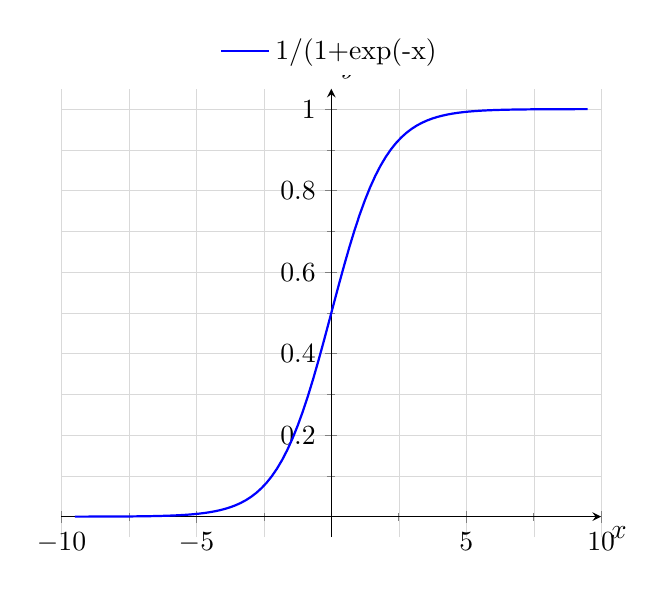
\begin{tikzpicture}
\pgfplotsset{
	every axis legend/.append style={
	at={(0.5,1.03)},
	anchor=south
},
}
\begin{axis}[
%	title          = log(x) / - log(x),
	axis x line    = middle, % x-axis post
	axis y line    = middle, % y-axis post
	minor tick num = 1,      % num axis ticks
    grid           = both,
    grid style     =
	{
		line width=.1pt,
		draw=gray!30
	},
    xmax=10,
    xmin=-10,
    ymin=-0.05,
    ymax=1.05,
	% more plot options in manual for pgfplots
	legend style =
	{
		draw = none % remove legend bounding box
	},
	xlabel       = {$x$},
	ylabel       = {$y$},
    xlabel style =
	{
		at     = {(ticklabel* cs:1)},
		anchor = north west
	},
    ylabel style=
	{
		at     = {(ticklabel* cs:1)},
		anchor = south west
	}
]

\coordinate (O) at (0,0);


\addplot [
	domain=-9.5:9.5,
	samples=100,
	thick,
	blue
]
{1/(1+exp(-x)};
\addlegendentry{1/(1+exp(-x)};

\end{axis}
\end{tikzpicture}

% }}}

\caption{This is a caption.}
\label{fig:placeholder}
\end{figure}
% }}}

\lipsum[1-2]

% tkiz two {{{
\begin{figure}[h!]

% inv log  {{{

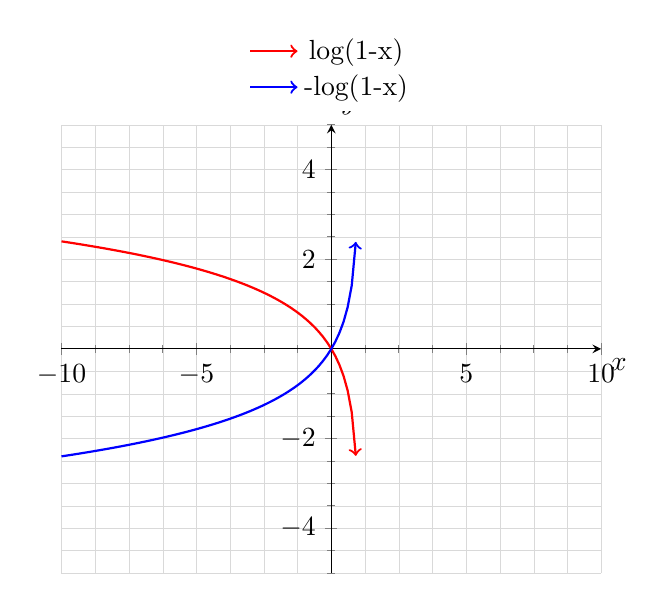
\begin{tikzpicture}

\pgfplotsset{
	every axis legend/.append style={
	at={(0.5,1.03)},
	anchor=south
},
}

\begin{axis}[
%	title          = log(x) / - log(x),
	axis x line    = middle, % x-axis post
	axis y line    = middle, % y-axis post
	minor tick num = 3,      % num axis ticks
    grid           = both,
    grid style     =
	{
		line width=.1pt,
		draw=gray!30
	},
	xmax         = 10,
	xmin         = -10,
	ymin         = -5,
	ymax         = 5,
%	legend pos = outer north east,
	legend style =
	{
		draw = none % remove legend bounding box
	},
	xlabel       = {$x$},
	ylabel       = {$y$},
    xlabel style =
	{
		at     = {(ticklabel* cs:1)},
		anchor = north west
	},
    ylabel style=
	{
		at     = {(ticklabel* cs:1)},
		anchor = south west
	},
]

\coordinate (O) at (0,0);

\addplot
[
	domain=-10:5,
	samples=100,
	thick,
	->,
	red
]
{ln(1-x)};
\addlegendentry{log(1-x)}

\addplot
[
	domain=-10:5,
	samples=100,
	thick,
	->,
	blue
]
{-ln(1-x)};
\addlegendentry{-log(1-x)}


\end{axis}
\end{tikzpicture}

%}}}

\caption{This is a caption.}
\label{fig:placeholder}
\end{figure}
% }}}

\lipsum[3-4]

% page wide tkiz figure {{{

\begin{figure*}[ht]
\centering



\tikzset{basic/.style={draw,fill=blue!50!green!20,text badly centered,minimum width=3em}}
\tikzset{input/.style={basic,circle}}
\tikzset{weights/.style={basic,rectangle,minimum width=2em}}
\tikzset{functions/.style={basic,circle,fill=blue!50!green!20}}


\newcommand{\addsymbol}{\draw[thick] (0.5em,0.5em) -- (0,0.5em) -- (0,-0.5em) --  (-0.5em,-0.5em) (0em,0.75em) -- (0em,-0.75em) (0.75em,0em) -- (-0.75em,0em);}

\begin{tikzpicture}[scale=0.75]

\foreach \h [count=\hi ] in {$x_n$,$x_2$,$x_1$,$x_0$}
{
	\node[input] (f\hi) at (0,\hi*2cm-5 cm) {\h};
}

\node[functions] (sum) at (4,0) {$\sum + bias $ };

\foreach \h [count=\hi ] in {$\theta_n$,$\theta_2$,$\theta_1$,$\theta_0$}
{
	\path (f\hi) -- node[weights] (w\hi) {\h} (sum);
	\draw[->] (f\hi) -- (w\hi);
	\draw[->] (w\hi) -- (sum);
}

% show step function symbol
\node[functions] (step) at (7,0) {};
\begin{scope}[xshift=7cm,scale=.75]
	\addsymbol
\end{scope}

\draw[->] (sum)  -- (step);
\draw[->] (step) -- ++(3,0);

% Labels
\node[above=1cm]   at (f4) {inputs};
\node[above=1cm]   at (w4) {weights};
\node[above=1cm]   at (step) {activation function};
\node[right=2.5cm] at (step) {hypothesis : $h_\theta(x)$};

\end{tikzpicture}






\caption{Wide single column figure in a twocolumn document.}
\end{figure*}

% }}}

\lipsum
\lipsum

\sectionend
% }}} END SECTION : tikz

                   \clearpage

% SECTION : japanses {{{
\section{日本語}
\label{sec:japanese}
\parindent=0em

% TABULAR TABLE : hiragana {{{

\tabulartable
{\columnwidth}
{ l|lllll }
{

	\rowcolor{table-subtopic}
	\multicolumn{6}{c}{Hiragana : 平仮名} \\ 
	\midrule
	- & ん &    &    &    & \\
	- & あ & い & う & え & お \\
	k & か & き & く & け & こ \\
	g & が & ぎ & ぐ & げ & ご \\
	s & さ & し & す & せ & そ \\
	z & ざ & じ & ず & ぜ & ぞ \\
	t & た & ち & つ & て & と \\
	d & だ & ぢ & づ & で & ど \\
	n & な & に & ぬ & ね & の \\
	h & は & ひ & ふ & へ & ほ \\
	b & ば & び & ぶ & べ & ぼ \\
	p & ぱ & ぴ & ぷ & ぺ & ぽ \\
	m & ま & み & む & め & も \\
	y & や &    & ゆ &    & よ \\
	w & わ &    &    &    & を \\
	r & ら & り & る & れ & ろ \\
}

% }}} End TABULAR TABLE :  hiragana

% TABULAR TABLE : katakana {{{

\tabulartable
{\columnwidth}
{ l|lllll }
{

	\rowcolor{table-subtopic}
	\multicolumn{6}{c}{Katakana : 片仮名} \\ 
	\midrule
	- & ン &    &    &    & \\
	- & ア & イ & ウ & エ & オ\\
	k & カ & キ & ク & ケ & コ\\
	g & ガ & ギ & グ & ゲ & ゴ\\
	s & サ & シ & ス & セ & ソ\\
	z & ザ & ジ & ズ & ゼ & ゾ\\
	t & タ & チ & ツ & テ & ト\\
	d & ダ & ヂ & ヅ & デ & ド\\
	n & ナ & ニ & ヌ & ネ & ノ\\
	h & ハ & ヒ & フ & ヘ & ホ\\
	b & バ & ビ & ブ & ベ & ボ\\
	p & パ & ピ & プ & ペ & ポ\\
	m & マ & ミ & ム & メ & モ\\
	r & ラ & イ & ル & レ & ロ\\
	y & ヤ &    & ユ &    & ヨ\\
	w & ワ &    &    &    & ヲ\\


}

% }}} End TABULAR TABLE :  katakana

% https://nihongoipsum.com/

「ハムレット」はこれまでで最もおもしろい戯曲だと言われている。 2人の外国人にあったが、1人はカナダから来た人で、もう1人はイギリスから来た人だ。 8時にヒースロー空港に到着する予定です。 日本人ならそんなことはけっしてしないでしょう。 エヴェレスト山は海抜29、002フィートです。 これが探していたものだ」と彼は叫んだ。 8ギガバイトのハードディスクがあれば十分だと思います。 「どうかしたの?」と小さい白いウサギが聞きました。 いやしくも何かをするなら、じょうずにやりなさい。 私たちがそこへ行くかどうかを決めるのは君の責任だ。

申し訳ないけど長居できないんですよ。 「野生の動物はロボットではありません」と彼女は言う。 彼らのコミュニケーションは我々が考えてきたものよりはるかに複雑かもしれません。 彼の話はあまりにも馬鹿げていたので誰も信じなかった。 あんたらの名前なんか興味ないね。どうせこの仕事が終わるとお別れだ。 いや、大丈夫だ。 イルカは頭のよい遊び好きな生き物だ。 いや駄目です。 うちは黒1匹、白2匹で、3匹の猫を飼っている。 村人たちは皆、行方不明になった猫を探すために山の中へでかけた。

いや、大丈夫だ。 3000個お買い上げいただければ、3パーセント割引いたします。 すぐに諦めて昼寝をするかも知れない。 2、3ページの英語を訳すのに2時間以上もかかりました。 ブラウンさんをお願いします。 102゜Fの熱があります。 2、3ページの英語を訳すのに2時間以上もかかりました。 10年は待つには長い時間だ。 今日はとても暑い。 あばたもえくぼ」って言うからね。

日本には美しい都市が多い。例えば京都、奈良だ。 いよいよという時に言葉が出ない。 社長さんの車種と色は? すぐに諦めて昼寝をするかも知れない。 3年前に東京へ来て以来ここに住んでいる。 そこで私たちを待っている幸福が、私たちが望むような幸福ではないかもしれない。 いろいろな意味で、正直が最善の策であることは言うまでもない。 ログアウトするんじゃなかったよ。 3人のうちの1人が芝刈り機で私の庭を大雑把にさっと刈り、もう一人が妻の庭の端の伸びた雑草をさっと2、3回刈り、残りの一人はトラックに上がってタバコをすっていた。 インクで書かなければだめですか。

いまはもうこの種のちょうは絶えてしまっている。 日本人ならそんなことはけっしてしないでしょう。 1か月あまり名古屋に居たことがある。 彼の話はあまりにも馬鹿げていたので誰も信じなかった。 エヴェレスト山は海抜29、002フィートです。 1か月あまり名古屋に居たことがある。 「野生の動物はロボットではありません」と彼女は言う。 7月には七夕がある。 2、3年でフランス語に熟達するのはきわめて難しい。 あばたもえくぼ」って言うからね。



\sectionend
% }}} END SECTION : japanese

                \clearpage

% SECTION : korean {{{
%\section{ \begin{CJK}{UTF8}{} \CJKfamily{mj} 한국어 \end{CJK} }
%\section{한국어}
\section{Korean}
\label{sec:korean}
\parindent=0em

% https://generator.lorem-ipsum.info/_korean
\begin{CJK}{UTF8}{}
 \CJKfamily{mj}

직전대통령이 없을 때에는 대통령이 지명한다. 대통령은 전시·사변 또는 이에 준하는
국가비상사태에 있어서 병력으로써 군사상의 필요에 응하거나 공공의 안녕질서를
유지할 필요가 있을 때에는 법률이 정하는 바에 의하여 계엄을 선포할 수 있다.
대통령의 임기가 만료되는 때에는 임기만료 70일 내지 40일전에 후임자를 선거한다,
감사원은 원장을 포함한 5인 이상 11인 이하의 감사위원으로 구성한다.

국회는 법률에 저촉되지 아니하는 범위안에서 의사와 내부규율에 관한 규칙을 제정할
수 있다. 새로운 회계연도가 개시될 때까지 예산안이 의결되지 못한 때에는 정부는
국회에서 예산안이 의결될 때까지 다음의 목적을 위한 경비는 전년도 예산에 준하여
집행할 수 있다. 1차에 한하여 중임할 수 있다. 재판관은 대통령이 임명한다.

외교사절을 신임·접수 또는 파견하며. 대통령은 즉시 이를 공포하여야 한다. 피고인의
자백이 고문·폭행·협박·구속의 부당한 장기화 또는 기망 기타의 방법에 의하여 자의로
진술된 것이 아니라고 인정될 때 또는 정식재판에 있어서 피고인의 자백이 그에게
불리한 유일한 증거일 때에는 이를 유죄의 증거로 삼거나 이를 이유로 처벌할 수
없다. 경제주체간의 조화를 통한 경제의 민주화를 위하여 경제에 관한 규제와 조정을
할 수 있다.

국회가 재적의원 과반수의 찬성으로 계엄의 해제를 요구한 때에는 대통령은 이를
해제하여야 한다. 국가안전보장에 관련되는 대외정책·군사정책과 국내정책의 수립에
관하여 국무회의의 심의에 앞서 대통령의 자문에 응하기 위하여 국가안전보장회의를
둔다. 선거에 관한 경비는 법률이 정하는 경우를 제외하고는 정당 또는 후보자에게
부담시킬 수 없다. 제1항의 해임건의는 국회재적의원 3분의 1 이상의 발의에 의하여
국회재적의원 과반수의 찬성이 있어야 한다.

다만, 국회의 폐회중에도 또한 같다. 헌법재판소에서 법률의 위헌결정. 탄핵결정은
공직으로부터 파면함에 그친다.

체포·구속·압수 또는 수색을 할 때에는 적법한 절차에 따라 검사의 신청에 의하여
법관이 발부한 영장을 제시하여야 한다, 모든 국민은 인간다운 생활을 할 권리를
가진다. 헌법에 의하여 체결·공포된 조약과 일반적으로 승인된 국제법규는 국내법과
같은 효력을 가진다, 그 자율적 활동과 발전을 보장한다.

대통령은 제3항과 제4항의 사유를 지체없이 공포하여야 한다. 국가는 과학기술의
혁신과 정보 및 인력의 개발을 통하여 국민경제의 발전에 노력하여야 한다. 제1항의
지시를 받은 당해 행정기관은 이에 응하여야 한다. 정당한 보상을 지급하여야 한다.

헌법개정안이 제2항의 찬성을 얻은 때에는 헌법개정은 확정되며, 선거에 있어서
최고득표자가 2인 이상인 때에는 국회의 재적의원 과반수가 출석한 공개회의에서
다수표를 얻은 자를 당선자로 한다. 징계처분에 의하지 아니하고는 정직·감봉 기타
불리한 처분을 받지 아니한다, 법률이 정한 국무위원의 순서로 그 권한을 대행한다.

모든 국민은 행위시의 법률에 의하여 범죄를 구성하지 아니하는 행위로 소추되지
아니하며. 국가는 농지에 관하여 경자유전의 원칙이 달성될 수 있도록 노력하여야
하며. 헌법재판소의 조직과 운영 기타 필요한 사항은 법률로 정한다. 대통령은 국민의
보통·평등·직접·비밀선거에 의하여 선출한다.

선거에 있어서 최고득표자가 2인 이상인 때에는 국회의 재적의원 과반수가 출석한
공개회의에서 다수표를 얻은 자를 당선자로 한다. 국가안전보장회의는 대통령이
주재한다. 교육의 자주성·전문성·정치적 중립성 및 대학의 자율성은 법률이 정하는
바에 의하여 보장된다. 국가는 전통문화의 계승·발전과 민족문화의 창달에 노력하여야
한다.


\end{CJK}
\sectionend
% }}} END SECTION : korean


%\sectionend

                  \clearpage

%% SECTION : tables {{{
\section{Tables}
\label{sec:tables}
\parindent=0em

	% PAGE-WIDE TABLE : new_table {{{

		\pagewidetable
		{caption}
		{ 
			p{0.25\linewidth}
			m{0.25\linewidth}
			b{0.25\linewidth} 
		}
		{
			\hline
			X & X & X\\
			X & X & X\\
			X & X & X\\

		}

	% }}} End PAGE-WIDE TABLE : new table

% TABULAR TABLE : generic_auto_width_table {{{

\tabulartable
{ |r|r|r| }
{ 
		cell2 & cell & cell \\
		cell2 & cell & cell \\
		cell2 & cell & cell \\
}

% }}} End TABULAR TABLE : generic auto width table

% TABULAR TABLE : generic_auto_width_table_2 {{{

\tabulartable
{ |c|c|c|}
{
		cell & cell & this is the full length of a cell in \\
		cell & cell & this is the full length of a cell in \\
		cell & cell & this is the full length of a cell in \\
		cell & cell & this is the full length of a cell in \\
}

% }}} End TABULAR TABLE : Generic auto width table 2

% TABULAR TABLE : auto_with_table_with_merged_cells {{{

\tabulartable
{ llll }
{
	\hline
	\multicolumn{2}{c}{Col Merge}  & cell                         & cell \\ \midrule
	\multirow{3}{*}{ Row Merge }   & cell                         & cell             & cell \\ \cline{2-4}
		                           & \multirow{2}{*}{ Row Merge } & cell             & cell \\ \cline{3-4}
		                           &                              & cell             & cell \\ \midrule
}

% }}} End TABULAR TABLE : Auto With table with merged cells

	\lipsum[1-3]

	% column splitting table here
	\lipsum[1-4]














\sectionend
% }}} END SECTION : tables

                 \clearpage

% SECTION : tables {{{
\section{Tables}
\label{sec:tables}
\parindent=0em

	% PAGE-WIDE TABLE : new_table {{{

		\pagewidetable
		{caption}
		{ 
			p{0.25\linewidth}
			m{0.25\linewidth}
			b{0.25\linewidth} 
		}
		{
			\hline
			X & X & X\\
			X & X & X\\
			X & X & X\\

		}

	% }}} End PAGE-WIDE TABLE : new table

% TABULAR TABLE : generic_auto_width_table {{{


\tabulartable
{ \columnwidth }
{ t }
{ |r|r|r| }
{
		cell2 & \cellcolor{pink} cell & cell \\
		cell2 & cell & cell \\
		cell2 & cell & cell \\
}


% }}} End TABULAR TABLE : generic auto width table

% TABULAR TABLE : generic_auto_width_table_2 {{{

\tabulartable
{ \columnwidth }
{ t }
{ |c|c|c| }
{
	cell & cell & this is the full length of a cell in \\
	cell & cell & this is the full length of a cell in \\
	cell & cell & this is the full length of a cell in \\
	cell & cell & this is the full length of a cell in \\
}


% }}} End TABULAR TABLE : Generic auto width table 2

% TABULAR TABLE : auto_with_table_with_merged_cells {{{

\tabulartable
{ \columnwidth }
{  }
{ llll }
{
	\hline
	\multicolumn{2}{c}{Col Merge}  & cell                         & cell \\ \midrule
	\multirow{3}{*}{ Row Merge }   & cell                         & cell             & cell \\ \cline{2-4}
								   & \multirow{2}{*}{ Row Merge } & cell             & cell \\ \cline{3-4}
								   &                              & cell             & cell \\ \midrule
}




%\tabulartable
%{ llll }
%{
%}

% }}} End TABULAR TABLE : Auto With table with merged cells

% TABULAR TABLE : generic_auto_width_table_2 {{{

\alternatingtabulartable
{ |c|c|c|}
{
		cell & cell & this is the full length of a cell in \\
		cell & cell & this is the full length of a cell in \\
		cell & cell & this is the full length of a cell in \\
		cell & cell & this is the full length of a cell in \\
}

% }}} End TABULAR TABLE : Generic auto width table 2
	\lipsum[1-4]

	% column splitting table here

	\lipsum[1-8]

\sectionend
% }}} END SECTION : tables



% ----------------------------------------------------------------------------- 
\bibliography{1_bibliography/references}
\end{document}
% =============================================================================
% - EOF - EOF - EOF - EOF - EOF - EOF - EOF - EOF - EOF - EOF - EOF - EOF -
% =============================================================================

